\documentclass[tikz]{standalone}
\usepackage{tikz}
\usepackage{fourier}
\usepackage{physics}
\usetikzlibrary{shapes.geometric}
\usetikzlibrary{calc}

\begin{document}
\begin{tikzpicture}
    % Spherical harmonic plots
    \node[inner sep=0] at (0, 0) {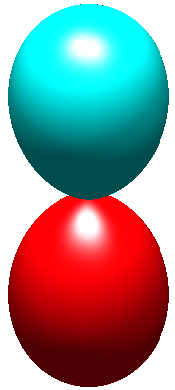
\includegraphics{../gfx/polar-spherical.pdf}};
    \node[inner sep=0] at (7, 0) {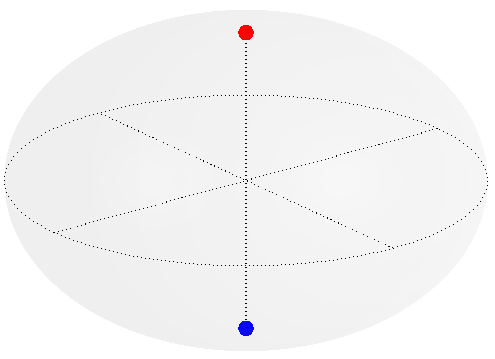
\includegraphics{../gfx/polar-Majorana.pdf}};
    \node[inner sep=0] at (16, 0) {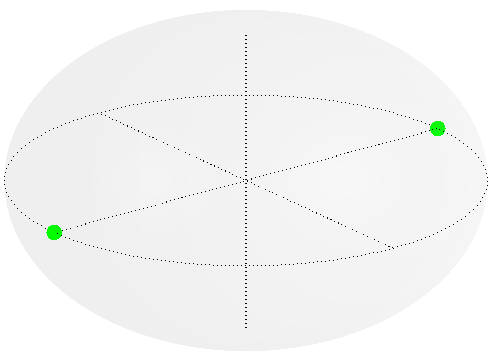
\includegraphics{../gfx/AFM-Majorana.pdf}};
         
    % Colour bar
    \node[rotate=90] at (-3.5, 0) {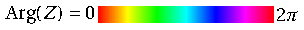
\includegraphics[scale=1.8]{../gfx/compiled_hsv.pdf}};
    \node at (21, 0) {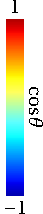
\includegraphics[scale=1.8]{../gfx/compiled_jet_majorana.pdf}};

    % Labels
    \node at (0, -4) {\LARGE (a)};
    \node at (7, -4) {\LARGE (b)};
    \node at (16, -4) {\LARGE (c)};

    % Polar labels
    \draw[-, line width=2] (0, 3.2) -- (0, 4.2) node[above] {\LARGE \(\hat{\vb{d}}\)};
    \draw[->, line width=2] (0.2, -0.05) -- (1.2, -0.05) node[right] {\LARGE \(C_2\)};

    % Orientation
    \draw[->, line width=2] (-2.8, -4) -- (-2.8, -3) node[above] {\LARGE \(z\)};
    \draw[->, line width=2] (-2.8, -4) -- (-1.8, -4) node[right] {\LARGE \(x\)};
    \draw[->, line width=2] (-2.8, -4) -- (-2.2, -3.5) node[right] {\LARGE \(y\)};

    % Spinor labels
    \node at (7, 3.5) {\LARGE \(\zeta^\text{EAP} = (0, 1, 0)^T\)};
    \node at (16, 3.5) {\LARGE \(\zeta^\text{EPP} = (1, 0, 1)^T/\sqrt{2}\)};

\end{tikzpicture}
\end{document}

